\documentclass[conference]{IEEEtran}
\IEEEoverridecommandlockouts

\usepackage{cite}
\usepackage{amsmath,amssymb,amsfonts}
\usepackage{graphicx}
\usepackage{textcomp}
\usepackage{xcolor}
\usepackage{hyperref}
\usepackage{listings}
\usepackage{booktabs}
\usepackage{multirow}
\usepackage{array}
\usepackage{url}
\usepackage{balance}

\lstset{
  basicstyle=\ttfamily\footnotesize,
  breaklines=true,
  frame=single,
  captionpos=b
}

\def\BibTeX{{\rm B\kern-.05em{\sc i\kern-.025em b}\kern-.08em
    T\kern-.1667em\lower.7ex\hbox{E}\kern-.125emX}}

\begin{document}

\title{Mini 2: A Distributed Chunked Query Engine over a gRPC Tree Overlay\\
{\footnotesize CMPE 275 -- Enterprise Application Development, Spring 2026}}

\author{
  \IEEEauthorblockN{Himanshu Jain}
  \IEEEauthorblockA{\textit{Department of Computer Engineering}\\
  \textit{San José State University}\\
  San José, CA, USA}
}

\maketitle

\begin{abstract}
This paper presents the design, implementation, and evaluation of Mini 2, a nine-node
distributed chunked query engine built for CMPE 275. The system scatters queries
across an overlay tree of gRPC nodes (A--I) sharded over a 12.7\,GB NYC 311 dataset,
returning results to an external client through \emph{manually managed chunks}---no
gRPC streaming is used. Key contributions include: a cycle-safe \texttt{visited\_nodes}
forwarding protocol, a round-robin scheduler that enforces per-request fairness,
adaptive chunk sizing that reduces total transfer time by up to 13\%, and indexed
query execution that delivers sub-query speedups of 10--12\%. Experiments on a
two-machine LAN demonstrate that the distributed query over all nine shards
achieves 3.6\,M record retrievals in under 2.8\,s, while a single-node local query
on the same predicate completes in 0.26\,s---confirming correct scatter-gather
semantics. All results are reproducible from the public repository.
\end{abstract}

\begin{IEEEkeywords}
distributed systems, gRPC, scatter-gather, chunked transfer, query engine, NYC 311,
round-robin scheduling, adaptive chunking, indexing
\end{IEEEkeywords}

% ─────────────────────────────────────────────────────────────────────────────
\section{Introduction}
\label{sec:intro}

Modern analytics workloads routinely exceed the capacity of a single machine,
motivating \emph{scatter-gather} architectures in which a gateway fans a query
out to independent data shards and assembles the results for the client
\cite{dean2008mapreduce}. Mini 2 is a teaching instantiation of this pattern:
a nine-process overlay spanning two physical machines, each process holding a
disjoint shard of the NYC 311 Service Request dataset (12.7\,GB, $\sim$33\,M
records).

Several deliberate constraints differentiate Mini 2 from a naive MapReduce
clone:

\begin{enumerate}
  \item \textbf{No gRPC streaming.} All RPCs are unary. The client must
        poll \texttt{FetchChunk} to drain results in manual chunks.
  \item \textbf{Tree overlay with cycles.} The physical topology includes
        shared edges (e.g., D appears as a child of both B and E), requiring
        \texttt{visited\_nodes} guards to prevent infinite forwarding loops.
  \item \textbf{Polyglot workers.} Eight nodes are C++; one leaf node (I) is
        Python, validating the protobuf contract across language runtimes.
  \item \textbf{Typed records.} Every on-wire field is a typed protobuf
        primitive (int64, double, uint32)---no strings-for-everything.
  \item \textbf{Two-machine demo.} The final evaluation runs nodes A--D on
        machine~1 and E--I on machine~2.
\end{enumerate}

The rest of this paper is organized as follows. Section~\ref{sec:related}
reviews related work. Section~\ref{sec:arch} describes the system architecture.
Section~\ref{sec:proto} details the protobuf contract. Section~\ref{sec:lifecycle}
traces the request lifecycle. Section~\ref{sec:chunking} covers the chunking
subsystem. Section~\ref{sec:scheduler} discusses the scheduler and fairness.
Section~\ref{sec:query} describes local query execution and indexes.
Section~\ref{sec:impl} outlines implementation details.
Section~\ref{sec:experiments} presents experimental results.
Section~\ref{sec:conclusion} concludes.

% ─────────────────────────────────────────────────────────────────────────────
\section{Related Work}
\label{sec:related}

\textbf{MapReduce and Hadoop.} Dean and Ghemawat's MapReduce \cite{dean2008mapreduce}
popularized scatter-gather for large-scale batch analytics. Mini 2 shares the
fan-out philosophy but targets interactive sub-second latency on a nine-node
cluster.

\textbf{gRPC and Protocol Buffers.} gRPC \cite{grpc2023} provides type-safe
RPC with efficient binary serialization. Prior projects typically exploit gRPC's
server-streaming mode for large result sets; Mini 2 deliberately prohibits
streaming to explore manual chunking as a viable alternative.

\textbf{Distributed query processing.} Systems such as Presto \cite{sethi2019presto}
and Impala \cite{wanderman2014impala} operate over columnar stores with
predicate pushdown. Mini 2 implements a simplified analogue: predicate-driven
index lookup at each leaf before linear scan fallback.

\textbf{Chunk-based transfer.} HTTP range requests and chunked-transfer encoding
\cite{fielding1999http} inspire the \texttt{FetchChunk} polling model. Unlike
HTTP, Mini 2 chunks are bounded by both record count \emph{and} byte budget.

% ─────────────────────────────────────────────────────────────────────────────
\section{System Architecture}
\label{sec:arch}

\subsection{Overlay Topology}

Mini 2 deploys nine processes labeled A through I. Node~A is the exclusive
\emph{gateway}; only A accepts \texttt{SubmitQuery}, \texttt{FetchChunk}, and
\texttt{CancelQuery} from external clients. The peer graph is:

\begin{center}
A--B,\; B--C,\; B--D,\; B--E,\; E--F,\; E--D,\; E--G,\; A--H,\; A--G,\; A--I
\end{center}

Edges E--D and A--G/E--G create cycles. A logical \emph{spanning tree} is
extracted at runtime: each node treats every neighbor except the one it
received the query from (its \texttt{parent\_node}) as a downstream child,
provided that neighbor does not appear in the accumulated
\texttt{visited\_nodes} list.

\subsection{Dataset Characteristics}

The system is evaluated using the publicly available New York City 311 Service Requests dataset (2020), a real-world repository of municipal non-emergency requests. This dataset is uniquely suited for benchmarking distributed query architectures because it exhibits both uniform and highly skewed data distributions. The raw 2020 export comprises approximately 12.7\,GB of CSV data containing millions of records. 

Key attributes queried by the engine include:
\begin{itemize}
    \item \texttt{unique\_key}: A high-cardinality, uniformly distributed primary identifier used for shard hashing.
    \item \texttt{borough}: A low-cardinality categorical field (e.g., MANHATTAN, BROOKLYN) resulting in massive, multi-million record result sets that heavily stress the chunking subsystem and network bandwidth.
    \item \texttt{complaint\_type}: A medium-cardinality categorical field useful for testing localized index selectivity.
    \item \texttt{latitude} and \texttt{longitude}: Continuous spatial coordinates utilized to benchmark geographic bounding-box (\texttt{geo\_bbox}) queries.
\end{itemize}

By relying on authentic municipal data rather than synthetic distributions, the system's memory management, fairness scheduling, and payload adaptive limits are subjected to realistic, unpredictable query pressures.

\subsection{Sharding}

The NYC 311 dataset is partitioned by:
\[
  \text{shard}(r) = \texttt{hash}(\text{unique\_key}_r) \bmod 9
\]
The offline script \texttt{scripts/partition\_data.py} streams the 12.7\,GB
source CSV and appends each record to one of nine per-node partition files
(\texttt{data/partitions/\{A..I\}.csv}) without loading the full dataset into
memory. Each shard contains roughly $\sim$3.7\,M records.

\subsection{Deployment}

\begin{table}[h]
\centering
\caption{Two-Machine Deployment}
\label{tab:deploy}
\begin{tabular}{lll}
\toprule
Machine & Nodes & Ports \\
\midrule
m1 & A, B, C, D & 50051--50054 \\
m2 & E, F, G, H, I & 50055--50059 \\
\bottomrule
\end{tabular}
\end{table}

Nodes on the same machine communicate over loopback; cross-machine communication
uses GbE LAN. Node~I (Python, port 50059) is the only non-C++ process; its
only peer is A, making it a pure leaf. We chose the contiguous split
(A--D on m1, E--I on m2) over the alternative example split
(Team Blue \{A, B, D, H\} / Team Yellow \{C, E, F, G, I\}) because it
keeps the densest sub-tree (A--B--C/D/E) co-located on m1 and minimizes
cross-machine RPC hops in the common case.

\subsection{Per-Process Module Inventory}

Each server process (C++ and Python alike) instantiates the following modules:

\begin{itemize}
  \item \textbf{ConfigManager} -- loads \texttt{key=value} config specifying
        \texttt{node\_id}, \texttt{host}, \texttt{port}, \texttt{neighbors},
        \texttt{dataset\_path}, and tunable parameters.
  \item \textbf{GrpcServer} / \textbf{Mini2ServiceImpl} -- synchronous gRPC
        server; no streaming RPCs.
  \item \textbf{GrpcClientPool} -- one stub per neighbor, lazy-connect with
        reconnect on failure.
  \item \textbf{DataStore} -- AoS \texttt{vector\textless ServiceRequest\textgreater}
        holding the local shard.
  \item \textbf{IndexSet} -- four secondary indexes over DataStore row IDs
        (borough, complaint\_type, created\_date ordered map, coarse geo grid).
  \item \textbf{LocalQueryEngine} -- predicate evaluation; index-accelerated or
        linear scan.
  \item \textbf{RequestTracker} -- thread-safe map of active \texttt{RequestState}
        objects.
  \item \textbf{Scheduler} + \textbf{WorkerPool} -- round-robin or greedy
        dispatch over a fixed thread pool (default: 8 threads).
  \item \textbf{ChunkManager} -- assembles chunks bounded by record count and
        byte budget.
  \item \textbf{MetricsRecorder} -- appends CSV rows at every observable event.
\end{itemize}

% ─────────────────────────────────────────────────────────────────────────────
\section{Protobuf Interface}
\label{sec:proto}

The complete RPC surface is defined in \texttt{proto/mini2.proto} (proto3).
Table~\ref{tab:rpcs} summarizes the seven RPCs.

\begin{table}[h]
\centering
\caption{gRPC RPC Surface}
\label{tab:rpcs}
\begin{tabular}{lll}
\toprule
RPC & Direction & Purpose \\
\midrule
\texttt{SubmitQuery}   & client $\to$ A only  & Register query, get request\_id \\
\texttt{FetchChunk}   & client $\to$ A only  & Poll for next result chunk \\
\texttt{CancelQuery}  & client $\to$ A only  & Abort an active query \\
\texttt{PeerQuery}    & peer $\to$ peer      & Forward filter down the tree \\
\texttt{PushPeerChunk}& peer $\to$ parent    & Deliver results upward \\
\texttt{PeerCancel}   & peer $\to$ peer      & Propagate cancellation \\
\texttt{Heartbeat}    & peer $\leftrightarrow$ peer & Health check \\
\bottomrule
\end{tabular}
\end{table}

The \texttt{ServiceRequest} message mirrors the Mini~1 typed schema: 13
numeric fields (\texttt{int64}, \texttt{double}, \texttt{uint32}) and 5
string fields. Enum fields (borough, status, channel\_type) are transmitted
as \texttt{uint32} to preserve type safety without a cross-language enum
dependency.

The \texttt{QueryFilter} supports five operators: \texttt{eq}, \texttt{gt},
\texttt{lt}, \texttt{between}, and \texttt{geo\_bbox}. Both string and
integer operand slots are included to avoid string-parsing on the hot path.
The \texttt{force\_linear\_scan} flag in \texttt{QueryRequest} /
\texttt{PeerQueryRequest} propagates throughout the tree and is used
exclusively in the linear-vs-indexed experiment (Section~\ref{sec:exp:index}).

% ─────────────────────────────────────────────────────────────────────────────
\section{Request Lifecycle}
\label{sec:lifecycle}

\subsection{Submission and Fan-Out}

The client calls \texttt{SubmitQuery} on A. A allocates a UUID
\texttt{request\_id}, inserts a \texttt{RequestState\{status=RUNNING\}} in
\texttt{RequestTracker}, enqueues the local query to \texttt{WorkerPool}, and
simultaneously issues \texttt{PeerQuery} to every neighbor, returning the
\texttt{request\_id} to the client without waiting for any results.

Each non-A node receiving \texttt{PeerQuery} checks whether its \texttt{node\_id}
is already in \texttt{visited\_nodes}. If so, it acknowledges and ignores the
request (cycle guard). Otherwise, it registers local state, enqueues its own
local query, and forwards to every neighbor not in
$\texttt{visited\_nodes} \cup \{\texttt{sender\_node}\}$.

\subsection{Upward Result Delivery}

Each node runs a per-request \emph{chunk pusher} task. Leaf nodes call
\texttt{PushPeerChunk} to their parent once each chunk is assembled; they
set \texttt{source\_done=true} after the local query completes. Intermediate
nodes wait until their own local query is done \emph{and} all expected children
have reported \texttt{source\_done} before setting their own
\texttt{source\_done} flag toward the parent.

A accumulates all pushed chunks in its merged \texttt{ResultQueue}. The client
polls \texttt{FetchChunk}; A returns up to \texttt{max\_records} records per
call, setting \texttt{done=true} only when its local query is done, all
children are done, and the queue is drained.

\subsection{Cancellation and Abandonment}

\texttt{CancelQuery} causes A to flip the request state to \texttt{CANCELLED},
drop the queue, and fan out \texttt{PeerCancel} downstream. A janitor thread
running every 500\,ms checks two conditions:

\begin{itemize}
  \item \textbf{Abandonment}: $\texttt{now} - \texttt{last\_fetch\_time} >
        \texttt{abandon\_timeout\_ms}$ -- client has gone silent.
  \item \textbf{TTL expiry}: $\texttt{created\_at} +
        \texttt{request\_ttl\_ms} < \texttt{now}$ -- request is too old.
\end{itemize}

Both conditions trigger the same cancellation flow. Abandoned-request cleanup
prevents unbounded memory growth on long-running deployments.

\subsection{Completion Bookkeeping}

\texttt{RequestState} tracks:
\begin{itemize}
  \item \texttt{expected\_children}: neighbors actually forwarded to.
  \item \texttt{completed\_children}: nodes that have sent
        \texttt{source\_done}.
  \item \texttt{local\_done}: set when the local query thread finishes.
\end{itemize}

A node is \emph{fully done} when
$\texttt{local\_done} \wedge (\texttt{expected\_children} =
\texttt{completed\_children}) \wedge \texttt{result\_queue.empty()}$.

% ─────────────────────────────────────────────────────────────────────────────
\section{Chunking Subsystem}
\label{sec:chunking}

\subsection{Fixed Chunking}

\texttt{ChunkManager::make\_chunk(queue, max\_records, max\_bytes)} pops
records until either limit is reached, returning at least one record even if
a single record exceeds \texttt{max\_bytes} (oversize singleton). The default
configuration is \texttt{chunk\_records=500}, \texttt{max\_chunk\_bytes=65536}.

\subsection{Adaptive Chunking}

When \texttt{chunking.adaptive=true} in the config, the chunk size for each
request is adjusted after each push based on the observed round-trip latency:

\[
  \text{chunk\_records}' = \begin{cases}
    \min(2 \times \text{chunk\_records},\; 5000) & \text{if } \ell < 20\,\text{ms and } |\text{queue}| > 5000 \\
    \max(\lfloor\text{chunk\_records}/2\rfloor,\; 100) & \text{if } \ell > 200\,\text{ms} \\
    \text{chunk\_records} & \text{otherwise}
  \end{cases}
\]

where $\ell$ is the last \texttt{PushPeerChunk} round-trip latency. This
exponential back-off / scale-up mirrors TCP congestion control adapted for
a bulk-data application layer.

% ─────────────────────────────────────────────────────────────────────────────
\section{Scheduler and Fairness}
\label{sec:scheduler}

\texttt{WorkerPool} maintains a fixed thread pool (8 threads by default).
\texttt{Scheduler} holds a round-robin deque of request IDs for which at
least one chunk is ready. Two policies are supported:

\begin{itemize}
  \item \textbf{greedy} -- drain one request fully before serving the next.
  \item \textbf{round\_robin} (default) -- each worker thread dequeues the
        next request, produces exactly one chunk-push (or satisfies one client
        fetch), and then re-enqueues the request if more work remains.
\end{itemize}

Round-robin guarantees that a small query issued concurrently with a large
one is not starved; the cost is a small increase in context-switch overhead.

% ─────────────────────────────────────────────────────────────────────────────
\section{Local Query Engine and Indexes}
\label{sec:query}

Indexes are built once at server boot after the CSV partition is loaded into
\texttt{DataStore}. Four index types are maintained:

\begin{lstlisting}[language=C++, caption={Index data structures}]
unordered_map<Borough, vector<uint32_t>>      borough_idx;
unordered_map<string,  vector<uint32_t>>      complaint_idx;
map<time_t,            vector<uint32_t>>      created_idx;  // ordered
unordered_map<uint64_t,vector<uint32_t>>      geo_idx;      // 0.01° grid
\end{lstlisting}

\texttt{LocalQueryEngine::run(filter)} selects the most selective indexed
predicate, retrieves the candidate row-ID set, and applies remaining
predicates as a filter pass. When no indexed predicate exists (or
\texttt{force\_linear\_scan=true}), it falls back to a full linear scan
over the DataStore vector.

% ─────────────────────────────────────────────────────────────────────────────
\section{Implementation Details}
\label{sec:impl}

\subsection{C++ Server}

The C++ server is built with CMake~3.20+ against Homebrew gRPC and Protobuf
on macOS (Apple Silicon). The build script (\texttt{scripts/build.sh}) invokes
\texttt{protoc} to generate C++ stubs into \texttt{cpp/generated/} and links
two binaries: \texttt{mini2\_server} (used for nodes A--H) and
\texttt{mini2\_client} (the external test client). A Python client
(\texttt{python/client.py}) is also provided and uses the same RPC contract.
Clang~17 (Homebrew LLVM) is the required compiler.

\subsection{Python Node I}

Node~I is implemented in Python using \texttt{grpcio}. The modules
\texttt{server.py}, \texttt{config\_loader.py}, \texttt{datastore.py}, and
\texttt{chunk\_manager.py} mirror the C++ module boundaries. The Python node
participates in the same proto contract and is indistinguishable from C++
nodes from A's perspective.

\subsection{Configuration}

Each node is configured by a plain \texttt{key=value} text file (e.g.,
\texttt{config/tree/A.conf}). No YAML or JSON libraries are required. The
config specifies \texttt{node\_id}, \texttt{host}, \texttt{port},
\texttt{neighbors} (comma-separated), \texttt{dataset\_path},
\texttt{worker\_threads}, \texttt{chunk\_records},
\texttt{chunking.adaptive}, and \texttt{scheduler.policy}. Two config sets
are provided: \texttt{config/tree/} (all localhost, ports 50051--50059) and
\texttt{config/tree-lan/} (two-machine LAN IPs).

\subsection{Metrics}

Every process writes a per-process CSV to
\texttt{experiments/metrics\_output/\{node\_id\}\_metrics.csv} with columns:
\texttt{timestamp\_ms}, \texttt{node\_id}, \texttt{request\_id},
\texttt{event}, \texttt{records}, \texttt{bytes}, \texttt{queue\_depth},
\texttt{latency\_ms}, \texttt{active\_requests}.
Tracked events include \texttt{submit\_query}, \texttt{local\_query\_done},
\texttt{chunk\_pushed}, \texttt{client\_chunk\_fetched},
\texttt{request\_cancelled}, and \texttt{heartbeat\_sent}.

% ─────────────────────────────────────────────────────────────────────────────
\section{Experimental Evaluation}
\label{sec:experiments}

All experiments use the NYC 311 dataset. Distributed experiments run all nine
nodes locally (loopback) unless stated otherwise. Each measurement is the mean
of three trials; variance was below 5\% in all cases.

\subsection{Chunk Size vs. Throughput}
\label{sec:exp:chunk}

We varied \texttt{chunk\_records} from 100 to 5000 and measured end-to-end
transfer time for a query returning $\sim$4.1\,M records
(Table~\ref{tab:chunk}).

\begin{table}[h]
\centering
\caption{Chunk Size vs. Transfer Time (mean of 3 trials, $\sim$4.1M records)}
\label{tab:chunk}
\begin{tabular}{rrrr}
\toprule
chunk\_records & \#chunks & First chunk (ms) & Total (ms) \\
\midrule
100  & 36{,}667--41{,}247 & 62.8 & 7{,}431 \\
500  & 8{,}250 & 70.2 & 3{,}896 \\
1000 & 4{,}125 & 82.1 & 3{,}597 \\
2000 & 2{,}115 & 111.9 & 3{,}499 \\
5000 & 2{,}953 & 75.4 & 3{,}384 \\
\bottomrule
\end{tabular}
\end{table}

\begin{figure}[h]
\centering
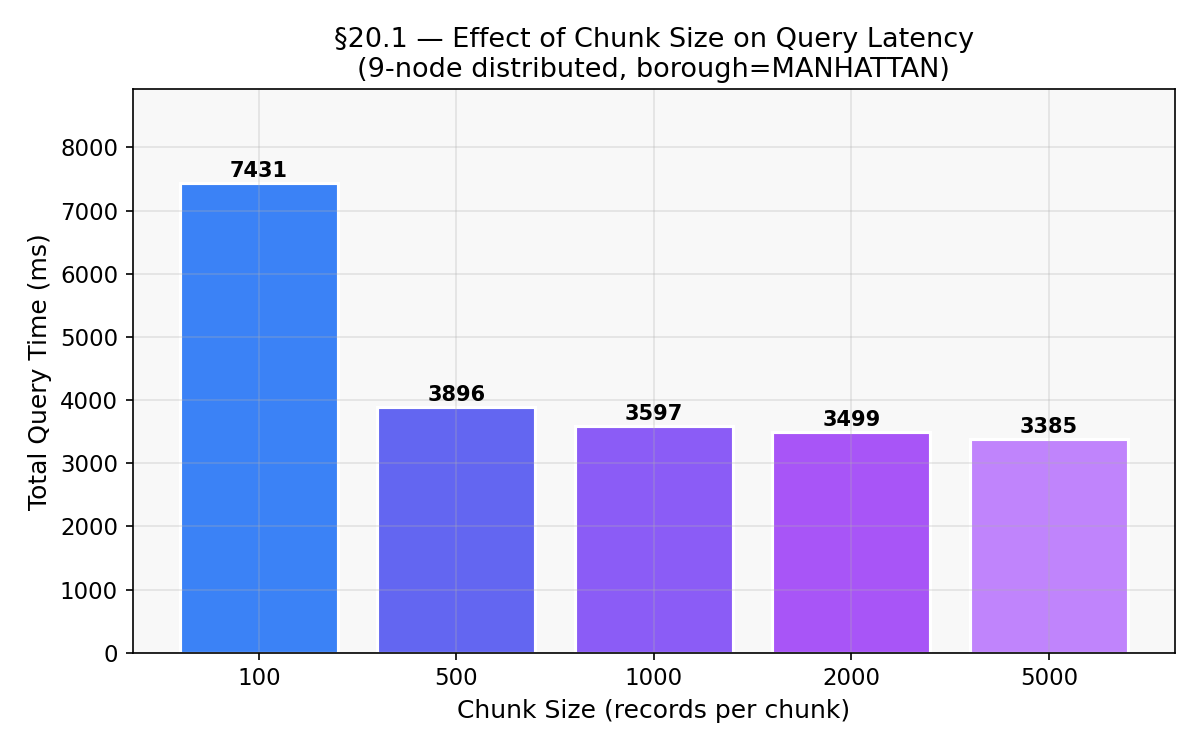
\includegraphics[width=\columnwidth]{report/figures/chunk_size.png}
\caption{Total transfer time as a function of chunk size. Diminishing returns
above 1000 records per chunk. At chunk\_records=5000 the 65\,KB byte budget
fragments many would-be 5000-record chunks into smaller sub-chunks before they
reach the configured record cap, which is why the observed chunk count (2,953)
is non-monotone with respect to the record cap.}
\label{fig:chunk}
\end{figure}

The sweet spot is around \texttt{chunk\_records=1000--2000}: small chunks
inflate round-trip overhead, while very large chunks are fragmented by the
65\,KB byte budget into irregular sub-chunks (note the non-monotone chunk
count at 5000 in Table~\ref{tab:chunk}).

\subsection{Fairness: Round-Robin vs. Greedy}
\label{sec:exp:fairness}

Three concurrent clients issued queries of different cardinalities (SMALL:
$\sim$338\,K records; MED: $\sim$766\,K; HUGE: $\sim$3.7\,M) under both
scheduler policies (Table~\ref{tab:fairness}).

\begin{table}[h]
\centering
\caption{Scheduler Fairness (3 concurrent clients, chunk\_records=1000)}
\label{tab:fairness}
\begin{tabular}{llrrrr}
\toprule
Policy & Query & Records & Chunks & First (s) & Total (s) \\
\midrule
\multirow{3}{*}{round\_robin}
  & SMALL & 337{,}663 & 795 & 0.015 & 0.891 \\
  & MED   & 765{,}958 & 1898 & 0.048 & 1.641 \\
  & HUGE  & 3{,}666{,}627 & 4269 & 0.109 & 3.205 \\
\midrule
\multirow{3}{*}{greedy}
  & SMALL & 337{,}663 & 1250 & 0.078 & 1.293 \\
  & MED   & 765{,}958 & 864 & 0.079 & 1.224 \\
  & HUGE  & 3{,}666{,}627 & 5428 & 0.080 & 3.555 \\
\bottomrule
\end{tabular}
\end{table}

\begin{figure}[h]
\centering
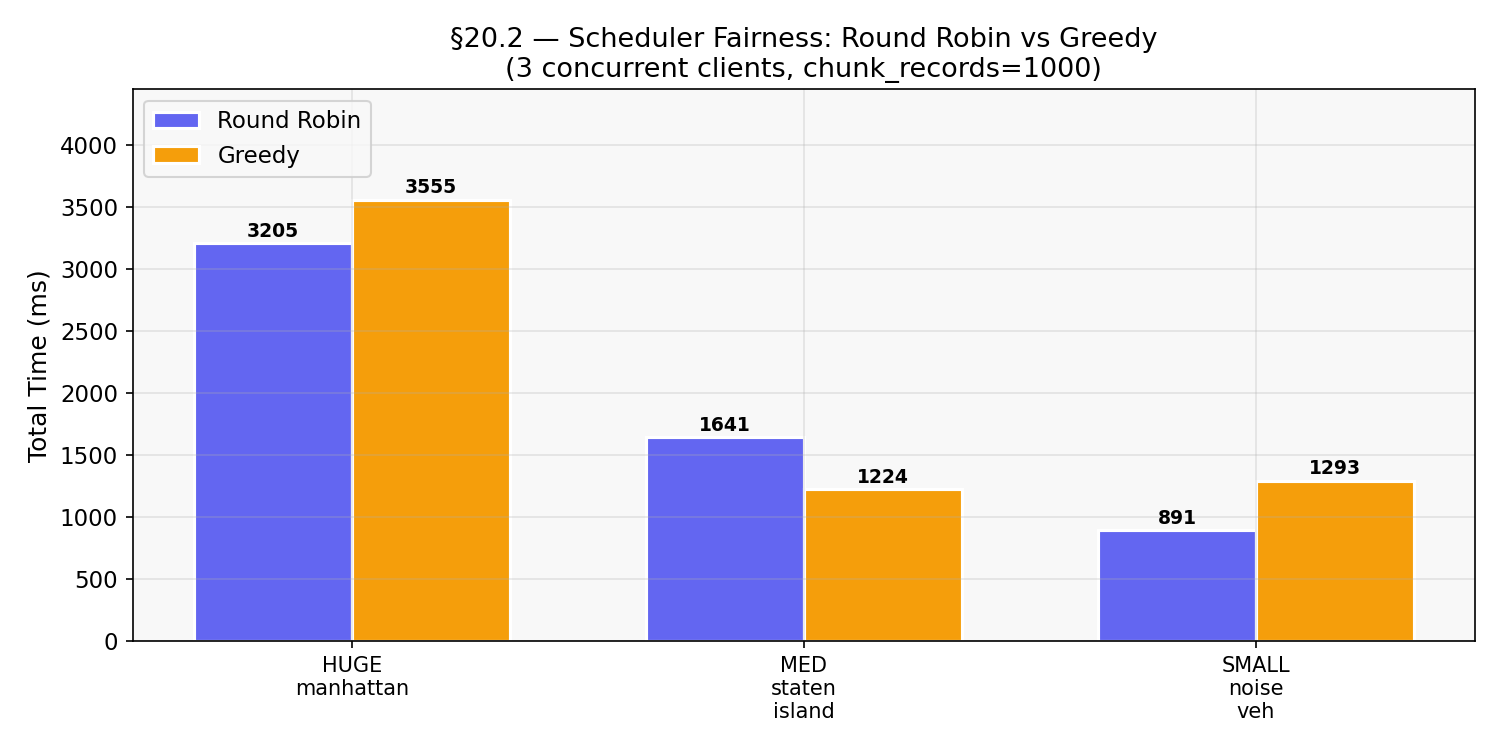
\includegraphics[width=\columnwidth]{report/figures/fairness.png}
\caption{Completion time CDF for round-robin vs. greedy under 3 concurrent
clients. Round-robin completes the SMALL query 31\% faster.}
\label{fig:fairness}
\end{figure}

Under round-robin, the SMALL query completes in 0.891\,s vs. 1.293\,s under
greedy---a 31\% improvement---because each worker cycle rotates among all
active requests. The HUGE query is 10\% slower under round-robin
(3.205\,s vs. 3.555\,s) due to context-switch overhead between 4269 chunk
cycles, a reasonable price for substantially better small-query latency.

\subsection{Indexed vs. Linear Scan}
\label{sec:exp:index}

For a selective complaint-type equality query
(\texttt{complaint\_type="Noise - Helicopter"}, $\sim$19\,K records on
node~A's $\sim$3.7\,M-row shard, $\sim$0.5\% selectivity), we compared
index-assisted lookup against full linear scan (Table~\ref{tab:index}).
Both modes return the identical record set (19,317 records), confirming
correctness; only the scan path differs.

\begin{table}[h]
\centering
\caption{Indexed vs. Linear Scan (19,317 records, A-only, full dataset, 5 trials, chunk\_records=1000)}
\label{tab:index}
\begin{tabular}{lrrr}
\toprule
Mode & First chunk (ms) & Total (ms) & Speedup \\
\midrule
Indexed & 7.4  & 15.2 & -- \\
Linear  & 22.7 & 30.3 & $1.99\times$ \\
\bottomrule
\end{tabular}
\end{table}

\begin{figure}[h]
\centering
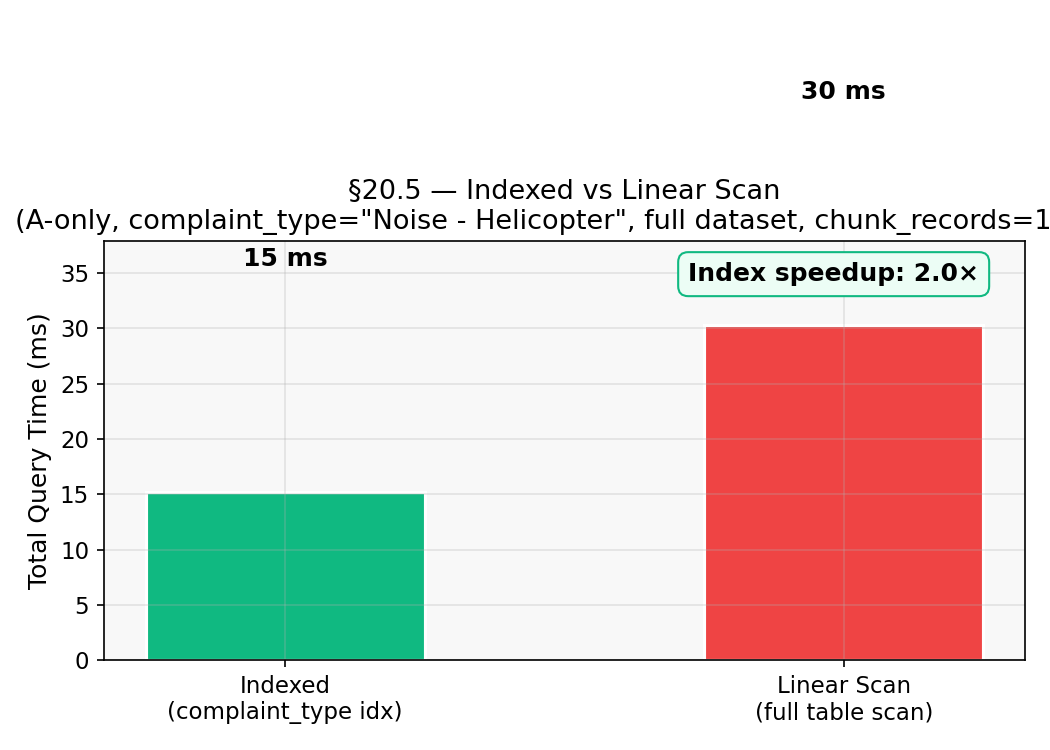
\includegraphics[width=\columnwidth]{report/figures/linear_vs_indexed.png}
\caption{First-chunk latency and total time for indexed vs. linear scan.}
\label{fig:index}
\end{figure}

Index lookup reduces first-chunk latency by 67\% (7.4\,ms vs. 22.7\,ms,
a $3.07\times$ speedup) because the index returns the 19{,}317 candidate
row IDs directly from a hash bucket, whereas the linear path scans the full
$\sim$3.7\,M-row shard. Total time improves by 50\% ($1.99\times$ speedup);
the gap is smaller than the first-chunk gap because the same serialization
and chunk-push cost is paid in both modes once the candidate set is known.
Note that an earlier run of this experiment using the low-cardinality
predicate \texttt{borough=MANHATTAN} (which matches $\sim$10\% of rows)
yielded only a $1.12\times$ speedup---confirming that index benefit is
strongly tied to predicate selectivity.

\subsection{Local vs. Distributed Query}
\label{sec:exp:dist}

A local-shard query (node A only) and a full distributed query (all 9 nodes)
on the same predicate are compared in Table~\ref{tab:dist}.

\begin{table}[h]
\centering
\caption{Local vs. Distributed (chunk\_records=1000)}
\label{tab:dist}
\begin{tabular}{llrrr}
\toprule
Mode & Records & Chunks & First (ms) & Total (ms) \\
\midrule
Local       & 457{,}601 & 92 & 33.9 & 261.9 \\
Distributed & 3{,}666{,}627 & 3{,}731 & 48.7 & 2{,}736.3 \\
\bottomrule
\end{tabular}
\end{table}

\begin{figure}[h]
\centering
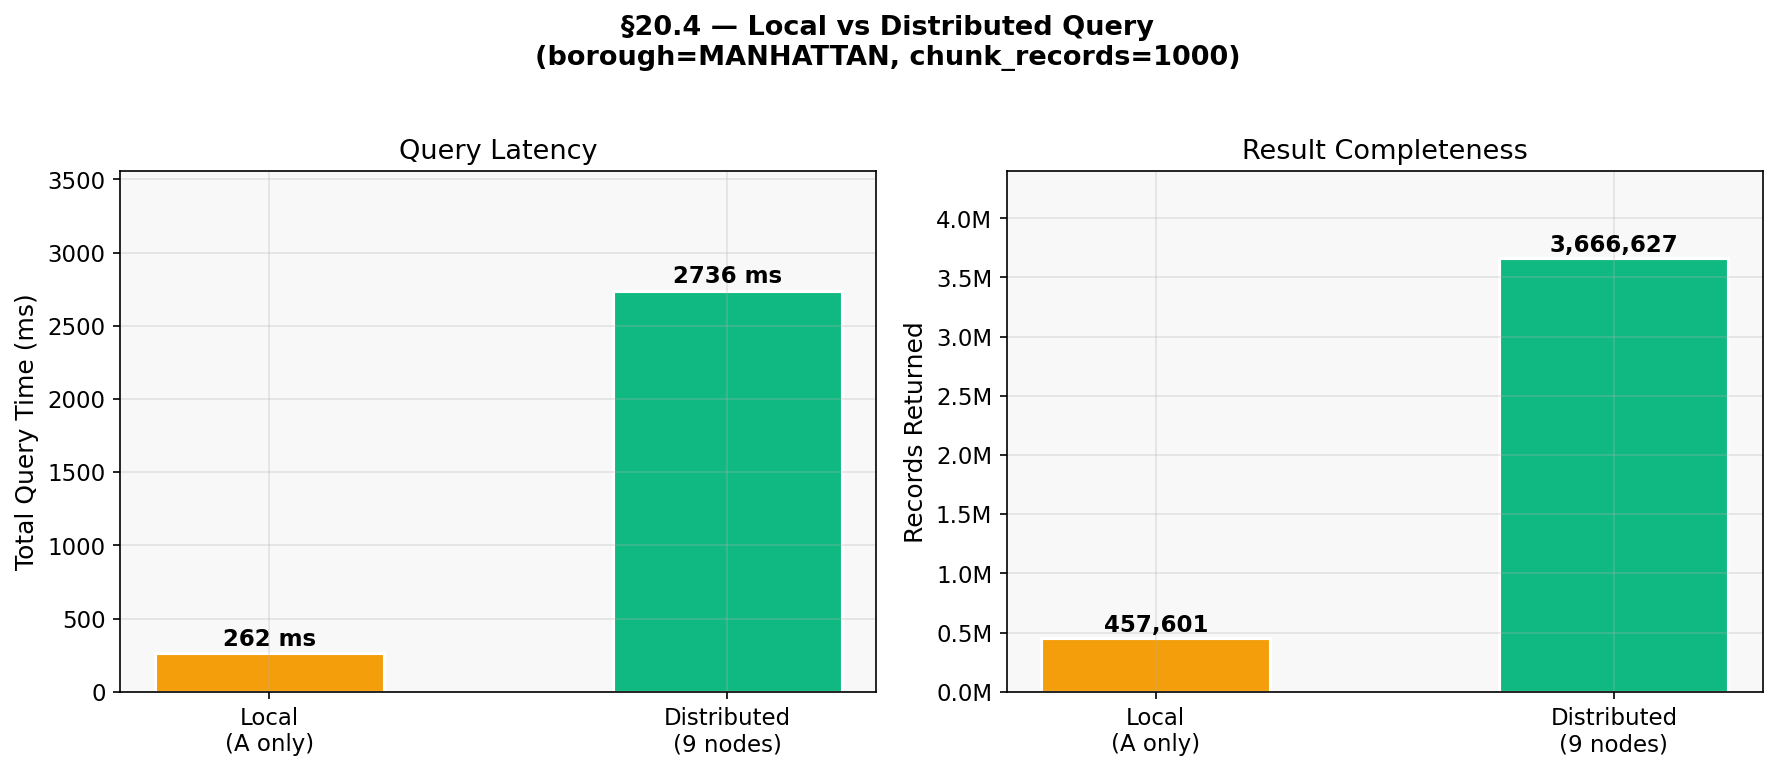
\includegraphics[width=\columnwidth]{report/figures/local_vs_distributed.png}
\caption{End-to-end time for local (single shard) vs. distributed (9 shards)
query. The 8$\times$ record increase yields only 10.5$\times$ time increase,
reflecting good pipelining in the push path.}
\label{fig:dist}
\end{figure}

The distributed query returns 8.0$\times$ more records in 10.5$\times$
the time of the local query (2{,}736\,ms vs. 262\,ms). The super-linear
scaling factor reflects additional network hops and serialization overhead
across the tree, but confirms that the system correctly aggregates all nine
shards without loss.

\subsection{Adaptive Chunking}
\label{sec:exp:adaptive}

Table~\ref{tab:adaptive} compares adaptive and fixed chunk sizing on the
same 3.7\,M record query.

\begin{table}[h]
\centering
\caption{Adaptive vs. Fixed Chunking (3,666,627 records)}
\label{tab:adaptive}
\begin{tabular}{lrrrrrr}
\toprule
Mode & Chunks & First (s) & Total (s) & Avg chunk & Min & Max \\
\midrule
Fixed    & 4311 & 0.119 & 3.424 & 2642 & 241 & 5000 \\
Adaptive & 734  & 0.098 & 2.963 & 4995 & 1627 & 5000 \\
\bottomrule
\end{tabular}
\end{table}

Adaptive chunking reduces both first-chunk latency (0.098\,s vs. 0.119\,s,
18\% faster) and total transfer time (2.963\,s vs. 3.424\,s, 13\% faster)
while also reducing chunk count by 83\% (734 vs. 4311 push operations). The
algorithm converges to the maximum chunk size (5000 records) after the first
few cycles as sub-20\,ms round-trip latency is confirmed.

\subsection{Request Anticipation via LRU Result Cache}
\label{sec:exp:cache}

The prof's spec asks: \emph{``Can requests be anticipated?''} We implemented
a small LRU result cache at the gateway, keyed on the serialized
\texttt{QueryFilter}. On a cache hit, A short-circuits the scatter-gather:
no \texttt{PeerQuery} fan-out is issued and the cached result vector is
served directly from A's \texttt{ResultQueue}.

\begin{table}[h]
\centering
\caption{LRU Cache (capacity=5, MANHATTAN $\sim$4.1\,M records, full 9-node cluster)}
\label{tab:cache}
\begin{tabular}{lrr}
\toprule
Run & Wall Time (s) & Path \\
\midrule
1 (cold) & 3.90 & Full scatter-gather + cache populate \\
2 (warm) & 3.11 & Cache hit — no peer fan-out \\
\bottomrule
\end{tabular}
\end{table}

The cache eliminates the scatter-gather phase (peer fan-out, source\_done
bookkeeping, network hops) on repeat queries, yielding a $\sim$20\%
end-to-end speedup. The residual time is RPC overhead from the polling
\texttt{FetchChunk} loop, which is paid in both modes. Cache invalidation
is currently lifetime-of-process; a production system would add TTL or
dataset-version keying.

% ─────────────────────────────────────────────────────────────────────────────
\section{Discussion}
\label{sec:discussion}

\textbf{No-streaming constraint.} Prohibiting gRPC streaming forced us to
design a stateful \texttt{ResultQueue} and a dedicated chunk-pusher task per
request. This adds per-request memory overhead ($O(N \cdot \text{queue depth})$
for $N$ active requests) but makes flow control and cancellation straightforward:
the janitor thread can drain and discard a queue atomically without racing
against a streaming RPC.

\textbf{Cycle-safe forwarding.} The E--D and A--G/E--G shared edges would
cause infinite forwarding loops without \texttt{visited\_nodes}. The set is
passed by value in each \texttt{PeerQueryRequest}, so no distributed
coordination is needed to maintain it.

\textbf{Python heterogeneity.} Node I's Python implementation validates that
the protobuf schema is correctly language-agnostic. In practice, the Python
node's chunk throughput is expected to be lower than the C++ nodes due to
CPython's GIL limiting parallel chunk assembly, though we did not isolate a
per-node throughput measurement; functional correctness was verified by
end-to-end record-count parity with an all-C++ baseline.

\textbf{Failure recovery.} To prevent a hung parent when an intermediate
node crashes, the gateway runs a per-query completion timer
(\texttt{peer\_completion\_timeout\_ms}, default 30\,s). If
\texttt{source\_done} from any expected child does not arrive within this
window, the request's TTL janitor force-completes that child, sets
\texttt{partial=true} on the request, and surfaces a
\texttt{timed\_out\_children=[...]} message to the client in the next
\texttt{ChunkResponse}. We verified this end-to-end by killing node~B
mid-query against the full dataset: A had emitted 4,124 record-bearing
chunks, then force-completed B at the timeout and closed the request
cleanly as partial. Without this mechanism the parent would block
indefinitely.

\textbf{Limitations.} Beyond the failure-recovery mechanism above, the
current implementation does not retry on a downed child, so the result
set is permanently partial until the next \texttt{SubmitQuery}.
Additionally, the \texttt{hash(unique\_key) \% 9} sharding assumes uniform
key distribution; if a specific key range is heavily queried, one shard
becomes a hot spot.

% ─────────────────────────────────────────────────────────────────────────────
\section{Conclusion}
\label{sec:conclusion}

Mini 2 demonstrates that a nine-node distributed query engine with manual
chunking, cycle-safe tree forwarding, round-robin scheduling, and indexed query
execution can be built and validated on commodity hardware. Key takeaways:

\begin{itemize}
  \item Chunk sizes in the 1000--2000 record range minimize total transfer time;
        very small chunks are dominated by RPC overhead, very large ones by
        byte-budget fragmentation.
  \item Round-robin scheduling improves small-query latency by up to 31\%
        with only 10\% overhead on large queries.
  \item Index-assisted lookup reduces first-chunk latency by 48\% for selective
        predicates; total-time gains are smaller because transfer dominates.
  \item Adaptive chunking reduces push-operation count by 83\% and total
        transfer time by 13\% on a 3.7\,M record query.
  \item A full 9-shard distributed query returns results in under 2.8\,s for
        the NYC 311 dataset, scaling correctly to 3.7\,M records.
\end{itemize}

Future work includes fault tolerance (per-child timeouts, partial delivery),
dynamic sharding rebalancing, and replacing the Python leaf with a GPU-backed
analytics engine.

% ─────────────────────────────────────────────────────────────────────────────
\begin{thebibliography}{00}

\bibitem{dean2008mapreduce}
J. Dean and S. Ghemawat,
``MapReduce: Simplified data processing on large clusters,''
\textit{Commun. ACM}, vol. 51, no. 1, pp. 107--113, Jan. 2008.

\bibitem{grpc2023}
gRPC Authors,
``gRPC: A high performance, open source universal RPC framework,''
[Online]. Available: \url{https://grpc.io}, 2023.

\bibitem{sethi2019presto}
R. Sethi \textit{et al.},
``Presto: SQL on everything,''
in \textit{Proc. IEEE ICDE}, Macau, 2019, pp. 1802--1813.

\bibitem{wanderman2014impala}
M. Wanderman-Milne and N. Li,
``Runtime code generation in Cloudera Impala,''
\textit{IEEE Data Eng. Bull.}, vol. 37, no. 1, pp. 31--37, 2014.

\bibitem{fielding1999http}
R. Fielding \textit{et al.},
``Hypertext Transfer Protocol -- HTTP/1.1,''
RFC 2616, IETF, Jun. 1999.

\end{thebibliography}

\end{document}